\subsection{Órbitas fechadas}
Nas discussões anteriores, foram analisadas trajetórias em anéis de armazenamento de elétrons com energia nominal $E_0$ --  a qual é a energia projetada para uma dada configuração ótica. No entanto, nem todos os elétrons armazenados possuem esta energia ideal. No geral, a energia $E$ de um elétron armazenado irá diferir da energia nominal, oscilando em torno desta. Estas oscilações de energia -- comumente chamadas de ''oscilações síncronas'' -- são o objeto de estudo desta seção.

Primeiramente, é necessário entender o movimento destes elétrons cuja energia difere de uma pequena quantidade $\epsilon$ da energia nominal. Mantendo a condição da \autoref{sec:3.2} de que a órbita ideal se encontra no plano horizontal, desvios de energia irão, para termos de primeira ordem, afetar apenas o movimento radial. O desvio vertical irá ser descrito apenas pelas oscilações betatron descritas na \autoref{part2}, e não serão consideradas nesta análise. Da \autoref{sec:2.6}, foi conveniente deixar que o símbolo $x$ representasse tanto $x_\beta$ quando $z_\beta$, os desvios laterais associados às oscilações betatron. A partir de agora, $x$ volta a representar o desvio horizontal total da trajetória com relação à órbita ideal.

Foi mostrado na \autoref{sec:2.5} que em um campo guia ideal o movimento radial de um elétron com um desvio de energia $\epsilon$ pode ser descrito pela soma de duas partes:
\begin{align}
	x = x_\beta + x_\epsilon
\end{align}
onde $x_\beta$ é o desvio causado pelas oscilações betatron e $x_\epsilon$ o desvio que depende apenas da energia do elétron. Acrescentando os resultados obtidos na \autoref{sec:2.11}, deve-se incluir o termo referente à distorção da órbita fechada devido às imperfeições magnéticas e escrever
\begin{align}
	x = x_\beta + x_\epsilon + x_c
\end{align}
Devido ao fato de que estes termos contribuem de forma linear -- assumindo um campo guia linear, pequenos desvios de energia e pequenas imperfeições magnéticas -- pode-se considerá-los separadamente. Agora, a análise será feita focando apenas em $x_\epsilon$.

De acordo com a equação \eqref{eq:2.28}, o desvio de energia pode ser escrito como
\begin{align}
	x_\epsilon = \eta(s)\frac{\epsilon}{E_0}\label{eq:3.3}
\end{align}
onde $\eta(s)$ é singularmente valorada em cada coordenada física $s$. Um elétron com energia diferente da nominal e sem oscilações betatron se move em uma nova órbita fechada onde seu desvio da órbita ideal é em todo lugar proporcional a $\epsilon/E_0$ com um fator de proporcionalidade que depende da coordenada $s$ pela função $\eta(s)$, função essa característica da configuração total do campo guia. A função $\eta(s)$ é chamada de função de dispersão, e é apenas o desvio da órbita fechada por unidade de desvio de energia.

Agora, deseja-se analisar a natureza de $\eta(s)$. $\eta(s)$ foi definida de forma que fosse a função única que satisfaz	
\begin{align}
	\begin{cases}
		\eta'' = -K_x(s)\eta + G(s), \\
        \eta(0) = \eta(L), \\
        \eta'(0) = \eta'(L).\label{eq:3.4}
    \end{cases}
\end{align}
As funções $G(s)$ e $K_x(s)$ foram definidas pelas equações \eqref{eq:2.3} e \eqref{eq:2.21}, respectivamente.

Agora, analisando o comportamento qualitativo implicado por esta definição para $\eta(s)$ de um campo guia de função separável (o qual foi definido na \autoref{sec:2.2}). Na \autoref{fig:fig29}(a),(b) estão representadas as funções $K_x$ e $G$ para um dado campo guia, e em (c) a função de dispersão $\eta(s)$.

\begin{figure}[!htb]
	\centering
	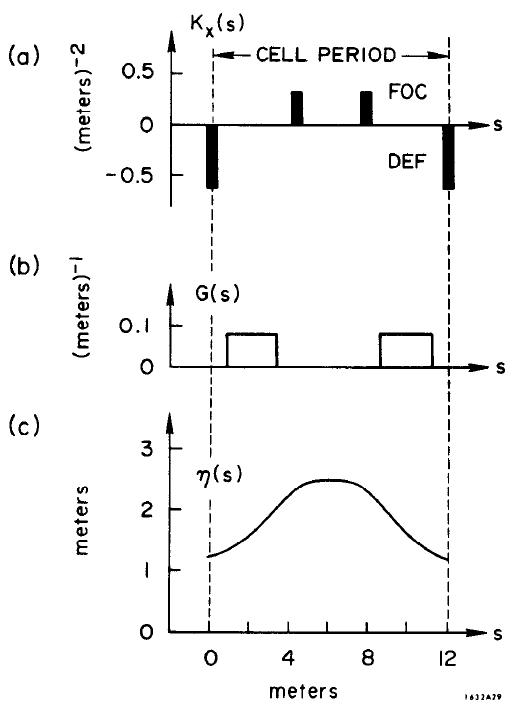
\includegraphics[width=0.6\linewidth]{./Figuras/fig29.jpeg}
	\caption{Funções do campo guia e a função de dispersão. Retirado de \cite{sands1970physics}.}
	\label{fig:fig29}
\end{figure}

Numa seção livre de campo, tanto $G$ quanto $K_x$ são nulas, então $\eta(s)$ tem um segmento com inclinação constante. Num quadrupolo puro, $G$ é zero e $K_x$ é apenas a força do quadrupolo. Num quadrupolo focalizador, $K_x$ é positivo e $\eta(s)$ segue uma oscilação senoidal em torno de zero na forma
\begin{align}
	\eta = a\ cos\left(\sqrt{K_x}s + \vartheta\right)
\end{align}
Em um quadrupolo desfocalizador, $K_x$ é negativo e $\eta(s)$ segue uma exponencial positiva na forma
\begin{align}
	\eta = a\ e^{(\sqrt{-K_x}s + \vartheta)}
\end{align}
A curva de $\eta(s)$ é "atraída" para o eixo $s$ em um quadrupolo focalizador e repelida do eixo em um quadrupolo desfocalizador.

Apesar de $K_1$ ser zero em um dipolo, $K_x$ não é. Na verdade, $K_x=G^2$ e a equação para $\eta$ fica
\begin{align}
	\eta'' = -G^2\eta + G = -G^2\left(\eta - \frac{1}{G}\right)
\end{align}

A curva de $\eta$ é um segmento senoidal o qual é "atraído" para $\eta_0 = 1/G$ com uma "força restauradora" proporcional a $G^2$ ($\eta_0$ é igual ao raio de curvatura $\rho$ da órbita ideal).

Da discussão acima, pode-se entender as características qualitativas das variações de $\eta(s)$ representadas na \autoref{fig:fig29}. Para todos os anéis de armazenamento "normais", a função de dispersão é positiva em todo o anel.

Considerando um campo guia de função separável, pode-se expandir a discussão anterior para calcular $\eta(s)$. Suponha que o cálculo inicie em $s=0$ assumindo alguns valores para $\eta(0)$ e $\eta'(0)$ e $\eta$ seja avaliada como uma sucessão de segmentos do tipo descrito anteriormente, até que seja feita uma revolução completa --  ou seja, até $s=L$. A verdadeira $\eta(s)$ será obtida se $\eta(0)$ e $\eta'(0)$ forem escolhidos de forma que $\eta(0) = \eta(L)$ e $\eta'(0) = \eta'(L)$. O cálculo pode ser computado utilizando uma técnica matricial.

A função de dispersão também pode ser obtida (para qualquer tipo de campo) utilizando os resultados obtidos na \autoref{sec:2.10} para as órbitas fechadas com distúrbio. Pode-se imaginar que a órbita fechada causada pela variação de energia é apenas uma órbita fechada com distúrbio, uma vez que tanto o desvio de energia quanto o erro de campo causam uma mudança na curvatura da trajetória. Em outras palavras, um erro de campo $\delta G$ em um segmento de órbita $\Delta s$ produz uma mudança na curvatura da trajetória de um elétron com energia $E_0$, mudança esta que é a mesma mudança na curvatura resultante de um desvio de energia $\epsilon$ de um elétron que viaja ao longo do campo nominal, já que $\delta G/G = \epsilon/E_0$. Já que $\eta(s)$ é a taxa do desvio da órbita fechada para $\epsilon/E_0$, pode-se computar $\eta(s)$ substituindo $\delta G$ na equação \eqref{eq:2.92} da \autoref{sec:2.11} por $G$. Este argumento também pode ser justificado notando que a equação \eqref{eq:3.4} para $\eta$ tem a mesma forma da equação \eqref{eq:2.85} para $x_c$ na \autoref{sec:2.10}; informalmente pode-se substituir $x_c \rightarrow \eta$ e $\delta G \rightarrow -G$. Fazendo estas substituições na equação \eqref{eq:2.94}, tem-se
\begin{align}
	\eta(s) = \frac{\sqrt{\beta(s)}}{2sen(\pi\nu)}\int\limits_{0}^{L}G(\bar{s})\sqrt{\beta(\bar{s})}cos(|\varphi(s)-\varphi(\bar{s})|-\pi\nu)d\bar{s}
\end{align}
Então, se $\beta(s)$ já é conhecido, pode-se obter $\eta(s)$ por uma integração. Note que $\eta(s)$ também terá um comportamento ressonante quando $\nu$ se aproxima de um inteiro.

Se a órbita ideal não está em um plano, esta discussão deve ser repetida para os desvios verticais. Neste caso, existirão duas funções de curvatura $G_x$ e $G_z$ assim como duas funções de focalização $K_x$ e $K_z$. Os desvios verticais também terão contribuições relativas ao desvio de energia, as quais serão proporcionais a função de dispersão $\eta_z(s)$. E a função de dispersão vertical pode ser avaliada em termos das funções de focalização e curvatura verticais. Terá apenas uma diferença qualitativa importante do caso horizontal: $\eta_z(s)$ terá tanto valores positivos quanto negativos, e sua média ao redor do anel será zero.